\paragraph{Sơ đồ tuần tự luồng đăng nhập / đăng ký bằng Google}

Luồng nghiệp vụ này mô tả
chi tiết
quá trình xác thực
và đăng nhập/đăng ký tài khoản thông qua dịch vụ bên thứ ba (Google).

\begin{figure}[H]
\centering
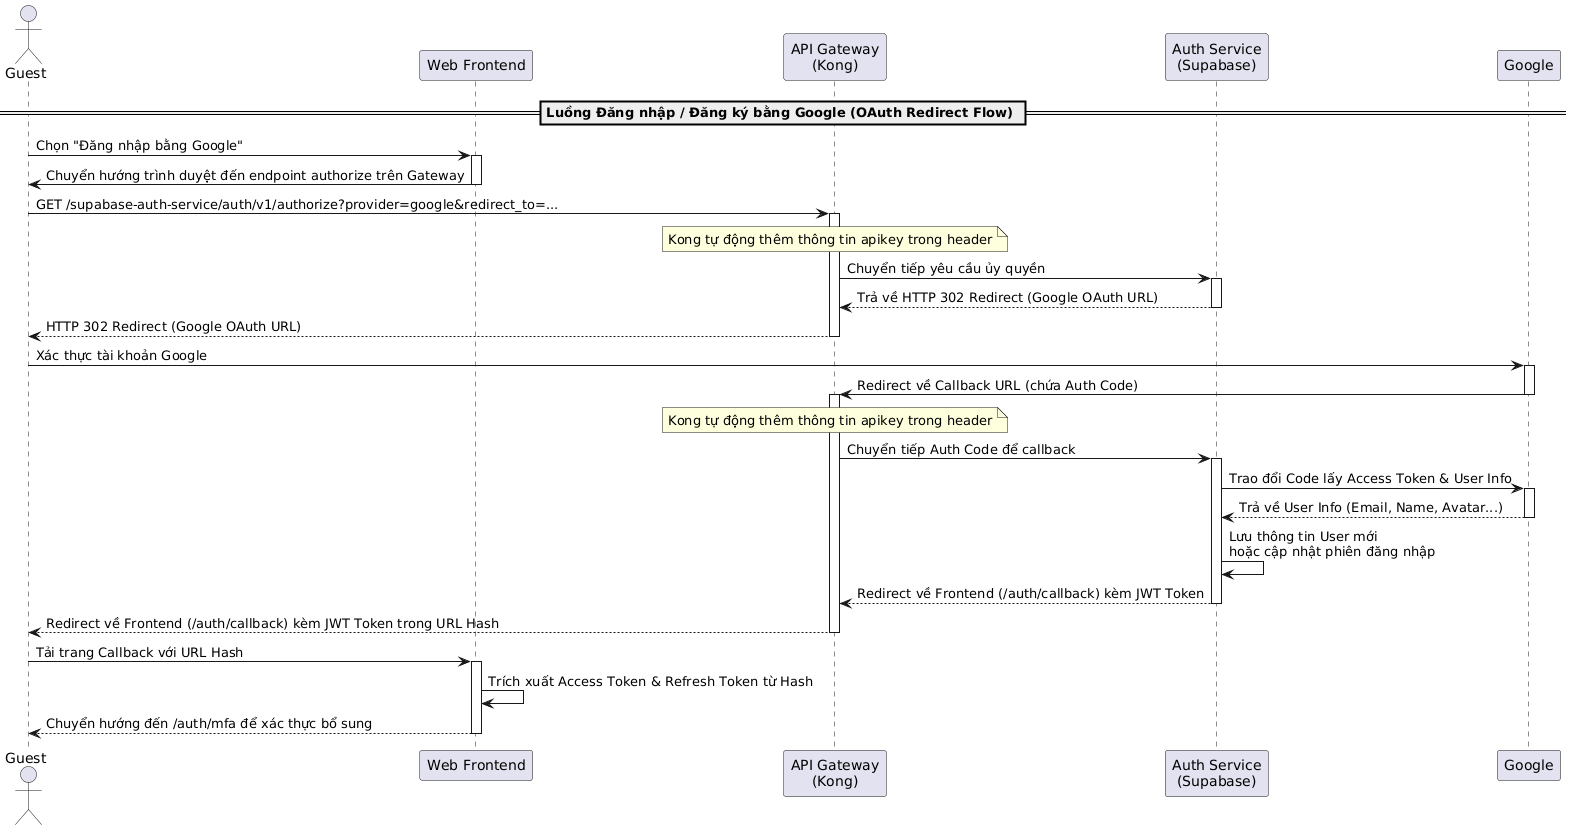
\includegraphics[width=0.95\textwidth]{contents/Sequence/UML-Sequence-GuestGoogleOAuthLogin.png}
\caption{Sơ đồ tuần tự luồng đăng nhập / đăng ký bằng Google}
\end{figure}

\begin{table}[H]
\centering
\renewcommand{\arraystretch}{1.3}

\begin{tabular}{|l|l|p{5cm}|}
\hline
\textbf{Thành phần} & \textbf{Phân loại} & \textbf{Vai trò trong hệ thống} \\ \hline
Guest & Actor & Khách vãng lai thực hiện đăng nhập hoặc đăng ký tài khoản. \\ \hline
Web Frontend & Component & Giao diện web Next.js. \\ \hline
API Gateway (Kong) & Component & Cổng API chuyển tiếp các yêu cầu API. \\ \hline
Auth Service (Supabase) & Microservice & Dịch vụ xác thực xử lý đăng ký, đăng nhập, giao tiếp Google và cấp phát JWT. \\ \hline
Google & External Service & Dịch vụ xác thực bên thứ ba của Google (OAuth 2.0). \\ \hline
\end{tabular}
\caption{Các thành phần tham gia luồng đăng nhập / đăng ký bằng Google}
\end{table}

\subparagraph{Mô tả tổng quan}

\begin{itemize}

\item \textbf{Chọn đăng nhập:}
Khách vãng lai chọn đăng nhập bằng tài khoản Google trên giao diện.
Giao diện chuyển hướng trình duyệt đến cổng API để gửi yêu cầu xác thực với Auth Service.

\item \textbf{Chuyển hướng trang đăng nhập:}
Auth Service phản hồi yêu cầu chuyển hướng người dùng sang trang đăng nhập của Google.
Trình duyệt tự động chuyển sang giao diện của Google để người dùng đăng nhập và cấp quyền.

\item \textbf{Nhận mã xác thực:}
Sau khi người dùng đồng ý,
Google chuyển hướng trình duyệt quay lại địa chỉ xử lý của Auth Service qua cổng API kèm theo mã xác thực tạm thời.

\item \textbf{Đổi mã lấy thông tin:}
Auth Service trao đổi mã này với Google để lấy thông tin tài khoản người dùng,
tiến hành tạo mới tài khoản (nếu là lần đầu)
hoặc cập nhật thông tin đăng nhập,
tạo mã phiên đăng nhập và mã làm mới,
sau đó chuyển hướng trình duyệt
về trang tiếp nhận của giao diện kèm các mã đăng nhập trong địa chỉ trang web.

\item \textbf{Lưu trữ mã đăng nhập:}
Giao diện trích xuất các mã này,
lưu trữ cục bộ
và chuyển hướng người dùng đến trang xác thực hai lớp
để hoàn tất xác minh trước khi vào màn hình chính.
\end{itemize}
